% Options for packages loaded elsewhere
\PassOptionsToPackage{unicode}{hyperref}
\PassOptionsToPackage{hyphens}{url}
\PassOptionsToPackage{dvipsnames,svgnames*,x11names*}{xcolor}
%
\documentclass[
  11pt,
]{article}
\usepackage{lmodern}
\usepackage{amssymb,amsmath}
\usepackage{ifxetex,ifluatex}
\ifnum 0\ifxetex 1\fi\ifluatex 1\fi=0 % if pdftex
  \usepackage[T1]{fontenc}
  \usepackage[utf8]{inputenc}
  \usepackage{textcomp} % provide euro and other symbols
\else % if luatex or xetex
  \usepackage{unicode-math}
  \defaultfontfeatures{Scale=MatchLowercase}
  \defaultfontfeatures[\rmfamily]{Ligatures=TeX,Scale=1}
\fi
% Use upquote if available, for straight quotes in verbatim environments
\IfFileExists{upquote.sty}{\usepackage{upquote}}{}
\IfFileExists{microtype.sty}{% use microtype if available
  \usepackage[]{microtype}
  \UseMicrotypeSet[protrusion]{basicmath} % disable protrusion for tt fonts
}{}
\makeatletter
\@ifundefined{KOMAClassName}{% if non-KOMA class
  \IfFileExists{parskip.sty}{%
    \usepackage{parskip}
  }{% else
    \setlength{\parindent}{0pt}
    \setlength{\parskip}{6pt plus 2pt minus 1pt}}
}{% if KOMA class
  \KOMAoptions{parskip=half}}
\makeatother
\usepackage{xcolor}
\IfFileExists{xurl.sty}{\usepackage{xurl}}{} % add URL line breaks if available
\IfFileExists{bookmark.sty}{\usepackage{bookmark}}{
\usepackage{hyperref}
}
\hypersetup{
  pdftitle={HTTP le protocole du Web},
  pdfauthor={Première NSI Lycée du Parc},
  colorlinks=true,
  linkcolor=Maroon,
  filecolor=Maroon,
  citecolor=Blue,
  urlcolor=Blue,
  pdfcreator={LaTeX via pandoc}}
\urlstyle{same} % disable monospaced font for URLs
\usepackage[top=20mm,left=20mm,right=20mm,heightrounded]{geometry}
\usepackage{listings}
\newcommand{\passthrough}[1]{#1}
\lstset{defaultdialect=[5.3]Lua}
\lstset{defaultdialect=[x86masm]Assembler}
\usepackage{longtable,booktabs}
% Correct order of tables after \paragraph or \subparagraph
\usepackage{etoolbox}
\makeatletter
\patchcmd\longtable{\par}{\if@noskipsec\mbox{}\fi\par}{}{}
\makeatother
% Allow footnotes in longtable head/foot
\IfFileExists{footnotehyper.sty}{\usepackage{footnotehyper}}{\usepackage{footnote}}
\makesavenoteenv{longtable}
\usepackage{graphicx}
\makeatletter
\def\maxwidth{\ifdim\Gin@nat@width>\linewidth\linewidth\else\Gin@nat@width\fi}
\def\maxheight{\ifdim\Gin@nat@height>\textheight\textheight\else\Gin@nat@height\fi}
\makeatother
% Scale images if necessary, so that they will not overflow the page
% margins by default, and it is still possible to overwrite the defaults
% using explicit options in \includegraphics[width, height, ...]{}
\setkeys{Gin}{width=\maxwidth,height=\maxheight,keepaspectratio}
% Set default figure placement to htbp
\makeatletter
\def\fps@figure{htbp}
\makeatother
\setlength{\emergencystretch}{3em} % prevent overfull lines
\providecommand{\tightlist}{%
  \setlength{\itemsep}{0pt}\setlength{\parskip}{0pt}}
\setcounter{secnumdepth}{5}

\title{HTTP le protocole du Web}
\author{Première NSI Lycée du Parc}
\date{}

%%%jolis boites

\usepackage{fancybox, graphicx}



%%%%%%%%%%%%%%%%Packages et Macros Frederic%%%%%%%%%%%%%%%%%%%%%%%%%%%%%


%%%%Insertion de liens hypertextes %%%%

            
%%%%%%%%%%PSTricks%%%%%%%%%%%%

\usepackage{pstricks,pst-plot,pst-text,pst-tree,pst-eps,pst-fill,pst-node,pst-math,pstricks-add,pst-xkey,pst-eucl}


%%%%%%%Tikz%%%%%%%%%%%%%%%
\usepackage{pgf,tikz,tkz-tab}
% Pour les tableaux de signes ou de variations avec tkz-tab voir https://zestedesavoir.com/tutoriels/439/des-tableaux-de-variations-et-de-signes-avec-latex/#1-13389_tikz-un-package-qui-en-a-dans-le-ventre
\usetikzlibrary{arrows}
\usetikzlibrary{shapes.geometric}
\usetikzlibrary{shapes.geometric}
\usetikzlibrary{petri}
\usetikzlibrary{decorations}
\usetikzlibrary{arrows}
\usetikzlibrary{math}
 %Variables must be declared in a tikzmath environment but
       % can be used outside
%       \tikzmath{int \n; \n = 508; \x1 = 1; \y1 =1; 
%                   %computations are also possible
%                    \x2 = \x1 + 1; \y2 =\y1 +3; } 


%%%%%%%%%%%%%%%%%%%%%%%%%%%%%%%%%%%%%%%%
%%%%%%%%%%%Commandes Tikz Perso%%%%%%%%%%%%%%%

% Définition des nouvelles options xmin, xmax, ymin, ymax
% Valeurs par défaut : -3, 3, -3, 3
\tikzset{
xmin/.store in=\xmin, xmin/.default=-3, xmin=-3,
xmax/.store in=\xmax, xmax/.default=3, xmax=3,
ymin/.store in=\ymin, ymin/.default=-3, ymin=-3,
ymax/.store in=\ymax, ymax/.default=3, ymax=3,
}
% Commande qui trace la grille entre (xmin,ymin) et (xmax,ymax)
\newcommand {\grille}[2]
{\draw[help lines,black, thick] (\xmin,\ymin) grid[xstep=#1, ystep=#2] (\xmax,\ymax);}
% Commande \axes
\newcommand {\axes} {
\draw[->,very thick] (\xmin,0) -- (\xmax,0);
\draw[->,very thick] (0,\ymin) -- (0,\ymax);
\draw (0.95*\xmax, 0) node[above] {};
\draw (0, 0.95*\ymax) node[left] {};
}
% Commande qui limite l?affichage à (xmin,ymin) et (xmax,ymax)
\newcommand {\fenetre}
{\clip (\xmin,\ymin) rectangle (\xmax,\ymax);}

%Exemple d'utilisation

%\begin{center}
%\begin{tikzpicture} [xmin=-2,xmax=2,ymin=0,ymax=5]
%\grille{1} \axes \fenetre
%\draw plot[smooth] (\x,\x^2);
%\end{tikzpicture}
%\end{center}

%style pour la perspective cavalière française
%voir Tikz pour l'impatient page 68
\tikzset{math3d/.style=
{x= {(-0.353cm,-0.353cm)}, z={(0cm,1cm)},y={(1cm,0cm)}}}

%%%%%%%Symbole pour code calculatrice%%%%%%

%Flèche remplie pour défilement de menu

\newcommand{\flechefillright}{

\begin{tikzpicture}[scale=0.15] \fill (0,0)--(2,1)--(0,2)--cycle;
\end{tikzpicture}}

%%%%%%%%%%%%%Symboles pour calculatrice Casio%%%%
\newcommand{\execasio}{\Pisymbol{psy}{191}} %Retour chariot
\newcommand{\dispcasio}{\begin{pspicture}(.1,.1)\pspolygon*(.1,0)(.1,.1)\end{pspicture}} %Triangle « Disp »
\newcommand{\dispcasiotikz}{
\begin{tikzpicture}[scale=0.2]
\fill (0,0) -- (1,0) -- (1,1) -- cycle;
\end{tikzpicture}} %Triangle « Disp »
%

%Fleche entre deux lignes, d'apres 'un bon petit' : http://forum.mathematex.net/latex-f6/fleches-entre-deux-lignes-pour-resolution-d-equation-t10283.html#p99817
\newcommand\addnode[1]{\Rnode{#1}{}}
\newcommand\linknode[3]{\ncbar[angleA=0,angleB=0,nodesep=1ex,arm=10ex,offset=-2pt]{->}{#1}{#2}\Aput{\vphantom{x}#3}}


%%Commande pour touche de calculatrice

\newcommand\tc[1]{%
{
\begin{tikzpicture}
\node[draw,rectangle,rounded corners=3pt] (P) at (0,0){#1};
\end{tikzpicture}
}
}

%%%%%%%%%%%%%%%%%%%%%%%%%%%%%%%%%%%%%%%%
%%%%%%%%%%%Fin Commandes Tikz%%%%%%%%%%%%%%%


%%%%%%%%%%%%Specifiques%%%%%%%%%%%
\usepackage{wrapfig}
%pour insérer une figure à droite ou à gauche d'un texte
%\begin{wrapfigure}[nb lignes]{placement l,r,c,i(inside),o(outside)}[overhang]{width}
%ce package fonctionne mal à proximité des listes
%%%%%%%%%%%%%%%%%%%%%%%%%%%%%%%%%%%%%

%%%%%Environnements et symboles spéciaux pour faire joli%%%%%%

%%%Bclogo, pour des environnements + jolis avec insertion de logo%%%%
%Dépendances de  bclogo
\usepackage{xkeyval}  
\usepackage{etoolbox}
\usepackage{ifpdf}
\usepackage[framemethod=tikz]{mdframed}
\usepackage[tikz]{bclogo}

%\newcommand\bcpython{\includegraphics[width=17pt]{/home/fjunier/Maths/python-logo.eps}}
\newcommand\bcpython{\includegraphics[width=17pt]{/home/fjunier/Maths/python-logo.png}}
%\newcommand\bcpython{\includegraphics[width=17pt]{/home/frederic/Maths/python-logo.png}}

%% Framed
\usepackage{framed}  %Le package « framed» Crée 3 nouveaux environnements, qui se comportent comme des minipage de largeur \linewidth, mais permettant en plus de se casser entre plusieurs pages.     * framed : avec un cadre autour;     * shaded : avec un fonc coloré (il faut définir la couleur shadecolor);     * leftbar : avec une barre le long du côté gauche.

%%%%%%%%%%%%%%%%%%%Présentation de codes sources%%%%%%%%%%%%%%%%%
\usepackage{listings}
%On utilise l?environnement lstlisting pour insérer
%un code source.
%En plus de l?environnement lstlisting, on peut également utiliser la
%commande \lstinline qui fonctionne comme la commande \verb, en ce
%sens qu?on peut utiliser n?importe quel caractère comme délimiteur. Enfin,
%la commande \lstinputlisting permet de charger un code source depuis
%un fichier externe.
%Il y a deux manières de préciser des options : soit via l?option de l?envi-
%ronnement ou de la commande, soit en utilisant la commande \lstset
%qui permet de définir des options de manière globale.

\lstset{ %
  language=Python,                % the language of the code
  basicstyle=\ttfamily,           % the size of the fonts that are used for the code
  %numbers=left,                   % where to put the line-numbers
  numberstyle=\tiny,  % the style that is used for the line-numbers
  %stepnumber=2,                   % the step between two line-numbers. If it's 1, each line 
                                  % will be numbered
  %numbersep=5pt,                  % how far the line-numbers are from the code
  backgroundcolor=\color{white},      % choose the background color. You must add \usepackage{color}
  showspaces=false,               % show spaces adding particular underscores
  showstringspaces=false,         % underline spaces within strings
  showtabs=false,                 % show tabs within strings adding particular underscores
  frame=single,                   % adds a frame around the code
  rulecolor=\color{black},        % if not set, the frame-color may be changed on line-breaks within not-black text (e.g. comments (green here))
  tabsize=4,                      % sets default tabsize to 2 spaces
  captionpos=b,                   % sets the caption-position to bottom
  breaklines=true,                % sets automatic line breaking
  breakatwhitespace=false,        % sets if automatic breaks should only happen at whitespace
  %title=\lstname,                   % show the filename of files included with \lstinputlisting;
                                  % also try caption instead of title
  breakindent=1cm,
  keywordstyle=\color{blue},          % keyword style
  commentstyle=\color{red},       % comment style
  %stringstyle=\ttfamily\color{green},         % string literal style
  escapeinside={\%*}{*)},            % if you want to add LaTeX within your code
  morekeywords={*,...},              % if you want to add more keywords to the set
  deletekeywords={...}              % if you want to delete keywords from the given language
  upquote=true,columns=flexible,
xleftmargin=1cm,xrightmargin=1cm,
 inputencoding=utf8,			%Les lignes qui suivent sont pour le codage utf8
  extendedchars=true,
  literate=%
            {é}{{\'{e}}}1
            {è}{{\`{e}}}1
            {ê}{{\^{e}}}1
            {ë}{{\¨{e}}}1
            {û}{{\^{u}}}1
            {ù}{{\`{u}}}1
            {â}{{\^{a}}}1
            {à}{{\`{a} }}1
            {î}{{\^{i}}}1
            {ô}{{\^{o}}}1
            {ç}{{\c{c}}}1
            {Ç}{{\c{C}}}1
            {É}{{\'{E}}}1
            {Ê}{{\^{E}}}1
            {À}{{\`{A}}}1
            {Â}{{\^{A}}}1
            {Î}{{\^{I}}}1
}

\lstdefinestyle{rond}{
  numbers=none,
  backgroundcolor=\color{gristclair},
  frameround =tttt
}

\lstdefinestyle{compil}{
  numbers=none,
  backgroundcolor=\color{gristclair}
}
%\lstset{language=Python,basicstyle=\small , frame=single,tabsize=4,showspaces=false,showtabs=false,showstringspaces=false,numbers=left,numberstyle=\tiny , extendedchars=true}



%%%%%%%%%%%%%%%%%%%%%%%%%%%%%%%%%%%%%%%%%%%%%%%%%%%%%%%%%%%%%%%%%%%%%%%%
%%%%%%%%%%%%%%%%%%%%Environnements persos%%%%%%%%%%%%%%%%%%%%%%%%%%%%%%%%
%Syntaxe :
%\newenvironment{nom}[nombre d'args][defaut]{definitions initiales}{definitions finales}
%definitions intiales sont les commandes appelées par \begin{nom}
%Definitions finales sont les commandes appelées par \end{nom}

%%%%%%%%%%%%%%%%Définitions des environnemts persostheoreme, exemple ..%%%%
%%%% Exercice avec encadré %%%%
\newcounter{exo}
\newenvironment{exercice}[1]
{\par \medskip   \addtocounter{exo}{1} \noindent  
\begin{bclogo}[arrondi =0.1,   noborder = true, logo=\bccrayon, marge=4]{~\textbf{Exercice} \textbf{\theexo} {\itshape #1} }  \par}
{
\end{bclogo}
 \par \bigskip }

%%Axiomes, Theoremes, Propriété, Définition, Methode, Preuve


\newenvironment{axiome}[1]
{\par \medskip   \begin{leftbar} \noindent \underline{\textbf{Axiome}}\hspace{0.5cm}{\itshape #1}   \vspace*{10pt} \par }
{\end{leftbar}  \par \medskip }


\newcounter{thme}
\newenvironment{theoreme}[1]
{\par \medskip  \addtocounter{thme}{1} \noindent  
\begin{bclogo}[arrondi =0.1,  ombre = true, barre=none, logo=\bcbook, marge=4]{~\textbf{Théorème} \textbf{\thethme} {\itshape #1} }   \par}
{
\end{bclogo}
 \par \bigskip}

 \newenvironment{theoremedef}[1]
{\par \medskip   \addtocounter{thme}{1} \noindent  
\begin{bclogo}[arrondi =0.1,  ombre = true, barre=none, logo=\bcbook, marge=4]{~\textbf{Théorème-Définition} \textbf{\thethme} {\itshape #1} }   \par}
{
\end{bclogo}
 \par \bigskip }
 
\newcounter{prop}
\newenvironment{propriete}[1]
{\par \medskip   \addtocounter{prop}{1} \noindent  
\begin{bclogo}[arrondi =0.1,  ombre = true, barre=none, logo=\bcbook, marge=4]{~\textbf{Propriété} \textbf{\theprop} {\itshape #1} }   \par}
{
\end{bclogo}
 \par \bigskip }


\newenvironment{corollaire}[1]
{\par \medskip   \noindent  
\begin{bclogo}[arrondi =0.1,  ombre = true, barre=none, logo=\bcbook, marge=4]{~\textbf{Corollaire} {\itshape #1} } \par }
{
\end{bclogo}
 \par \bigskip }

\newenvironment{demo}[1]
{\par \medskip   \noindent  
\begin{bclogo}[arrondi =0.1,  ombre = true, barre=zigzag, noborder = true, logo=\bcloupe, marge=0]{~\textbf{Démonstration} {\itshape #1} } \par \vspace{10pt}}
{
\end{bclogo}
 \par \bigskip }

\newcounter{activite}
\newenvironment{activite}[1]
{\par \medskip   \noindent   \addtocounter{activite}{1}
\begin{bclogo}[arrondi =0.1,   noborder = true, logo=\bcvelo, marge=4]{~\textbf{Activité} \textbf{\theactivite} {\itshape #1} }  \par}
{
\end{bclogo}
 \par \bigskip }


\newcounter{rque}
\newenvironment{remarque}
{\par \medskip    \addtocounter{rque}{1} \noindent  
\begin{bclogo}[arrondi =0.1,  ombre = true, barre=snake, noborder = true, logo=\bcinfo, marge=0]{~\textbf{Remarque} \textbf{\therque}}  \par }
{
\end{bclogo}
 \par \bigskip }

\newcounter{def}
\newenvironment{definition}[1]
{\par \medskip   \addtocounter{def}{1} \noindent  
\begin{bclogo}[arrondi =0.1,  ombre = true, barre=none, logo=\bcbook, marge=4]{~\textbf{Définition} \textbf{\thedef} {\itshape #1} }  \par}
{
\end{bclogo}
 \par \bigskip }
 
 
 \newcounter{cours}
\newenvironment{cours}[1]
{\par \medskip   \addtocounter{cours}{1} \noindent  
\begin{bclogo}[arrondi =0.1,  ombre = true, barre=none, logo=\bcbook, marge=4]{~\textbf{Point de cours} \textbf{\thecours} {\itshape #1} }  \par}
{
\end{bclogo}
 \par \bigskip }
 
 

\newcounter{exple}
\newenvironment{exemple}[1]
{\par \medskip   \addtocounter{exple}{1} \noindent  
\begin{bclogo}[arrondi =0.1,   noborder = true, logo=\bclampe, marge=4]{~\textbf{Exemple} \textbf{\theexple} {\itshape #1} }  \par}
{
\end{bclogo}
 \par \bigskip }




\newcounter{alg}
\newenvironment{algorithme}[1]
{\par \medskip   \addtocounter{alg}{1} \noindent  
 \begin {bclogo}[noborder = true, barre=zigzag,logo=\bcpython, marge=4] {~\textbf{Algorithmique} \textbf{\thealg} {\itshape #1} }  \par}
{
\end{bclogo}
 \par \bigskip }

\newcounter{prog}
\newenvironment{programme}[1]
{\par \medskip   \addtocounter{prog}{1} \noindent  
 \begin {bclogo}[noborder = true, barre=zigzag,logo=\bcpython, marge=4] {~\textbf{Programme} \textbf{\theprog} {\itshape #1} }  \par  \bigskip}
{
\end{bclogo}
 \par \bigskip }
 
\newcounter{logi}
\newenvironment{logique}[1]
{\par \medskip   \addtocounter{logi}{1} \noindent  
 \begin {bclogo}[noborder = true, barre=zigzag,logo=\bclampe, marge=4] {~\textbf{Logique} \textbf{\thelogi} {\itshape #1} }  \par}
{
\end{bclogo}
 \par \bigskip }


\newenvironment{methode}[1]
{\par \medskip    \noindent  
 \begin {bclogo}[arrondi =0.1,logo=\bcoutil, marge=4,noborder = true] {~\textbf{Méthode}   {\itshape #1} }  \par}
{
\end{bclogo}
 \par \bigskip }


\newcounter{histo}
\newenvironment{histoire}[1]
{\par \medskip   \addtocounter{histo}{1} \noindent  
 \begin {bclogo}[couleur = blue!10 , arrondi =0.1,logo=\bchorloge, marge=4] {~\textbf{Histoire} \textbf{\thehisto} {\itshape #1} }  \par}
{
\end{bclogo}
 \par \bigskip }




%Environnement contenu pour un document présentant une progression annuelle
\newenvironment{contenu}
{\par \medskip   \begin {bclogo}[ noborder = true,logo=\bccrayon] \noindent {\large \textbf{Contenu de la séance}} \vspace*{10pt} \par  }
{\end{bclogo}  \par \medskip }

%Environnement programme pour un document présentant une progression annuelle
%\newenvironment{programme}
%{\par \medskip   \begin {bclogo}[ noborder = true, barre=zigzag,logo=\bcinfo] \noindent {\large \textbf{Programme officiel}} \vspace*{10pt} \par  }
%{\end{bclogo}  \par \medskip }

%Environnement programme pour un document présentant une progression annuelle
\newenvironment{ressource}
{\par \medskip   \begin {bclogo}[ noborder = true,logo=\bcbook] \noindent {\large \textbf{Ressources}}\\vspace*{10pt} \par }
{\end{bclogo}  \par \medskip }




%%%%%%%%%%%%%%%%%%Maths divers%%%%%%%%%%%%%%%%%%%%%%%%%
%%%%%%%%%%%%%Nombres%%%%%%%%%%%%%%%%

%Ensemble prive de...
%\newcommand{\prive}{\boi}%{\backslash}

%Ensembles de nombres%%%%%%%%%%%%%%%%%
\newcommand{\R}{\mathbb{R}}
\newcommand{\N}{\mathbb{N}}
\newcommand{\D}{\mathbb{D}}
\newcommand{\Z}{\mathbb{Z}}
\newcommand{\Q}{\mathbb{Q}}
%\newcommand{\C}{\mathbb{C}}
\newcommand{\df}{~\ensuremath{]0;+\infty[}~}
\newcommand{\K}{\mathbb{K}}

%%%%%%%%Arithmetique%%%%%%%%%%
%PGCD, PPCM
\newcommand{\PGCD}{\mathop{\rm PGCD}\nolimits}
\newcommand{\PPCM}{\mathop{\rm PPCM}\nolimits}

%Intervalles
\newcommand{\interoo}[2]{]#1\, ;\, #2[}
\newcommand{\Interoo}[2]{\left]#1\, ;\, #2\right[}
\newcommand{\interof}[2]{]#1\, ;\, #2]}
\newcommand{\Interof}[2]{\left]#1\, ;\, #2\right]}
\newcommand{\interfo}[2]{[#1\, ;\, #2[}
\newcommand{\Interfo}[2]{\left[#1\, ;\, #2\right[}
\newcommand{\interff}[2]{[#1\, ;\, #2]}
\newcommand{\Interff}[2]{\left[#1\, ;\, #2\right]}
%\newcommand\interentiers #1#2{[\! [#1\, ;\, #2]\! ]}
\newcommand{\interentiers}[2]{\llbracket #1\, ;\, #2\rrbracket}
%


%%%%%%%%%%%%%%Nombres complexes%%%%%

\newcommand{\ic}{\text{i}}
%\newcommand{\I}{\text{i}}
\newcommand{\im}[1]{\text{Im}\left(#1\right)}
\newcommand{\re}[1]{\text{Re}\left(#1\right)}
\newcommand{\Arg}[1]{\text{arg}\left(#1\right)}
\newcommand{\Mod}[1]{\left[#1\right]}
%Parties entière, réelle, imaginaire, nombre i
\newcommand{\ent}[1]{\text{E}\left(#1\right)}
\renewcommand{\Re}{\mathop{\rm Re}\nolimits}
\renewcommand{\Im}{\mathop{\rm Im}\nolimits}
\renewcommand{\i}{\textrm{i}}

%%%%%%%%%%%Probabilites et statistiques%%%%%
\newcommand{\loibinom}[2]{\mathcal{B}\left(#1\ ; \ #2 \right)}
\newcommand{\loinorm}[2]{\mathcal{N}\left(#1\ ; \ #2 \right)}
\newcommand{\loiexp}[1]{\mathcal{E}\left(#1\right)}
\newcommand{\proba}[1]{\mathbb{P}\big(#1\big)}
\newcommand{\probacond}[2]{\mathbb{P}_{#2}\big(#1\big)}
\newcommand{\esperance}[1]{\mathbb{E}\left(#1\right)}
\newcommand{\variance}[1]{\mathbb{V}\left(#1\right)}
\newcommand{\ecart}[1]{\sigma\left(#1\right)}
\newcommand{\dnormx}{\frac{1}{\sqrt{2\pi}} \text{e}^{-\frac{x^2}{2}}}
\newcommand{\dnormt}{\frac{1}{\sqrt{2\pi}} \text{e}^{-\frac{t^2}{2}}}

%Covariance
\newcommand{\cov}{\mathop{\rm cov}\nolimits}
%


%%%%%%%%%%Analyse%%%%%%%%%%%

%%%%%%%%%%%Courbe%%%%%%%%%%%%
\newcommand{\courbe}[1]{\ensuremath{\mathcal{C}_{#1}}}

%%%%%%%Fonction exponentielle%%%%%
\newcommand{\fe}{~fonction exponentielle~}
\newcommand{\e}{\text{e}}

%Fonction cotangente
\newcommand{\cotan}{\mathop{\rm cotan}\nolimits}
%%%%%%%%%%%%%%%%%%%%%%%%%%%%%%%%%%%%%%%%%
%
%Fonctions hyperboliques
\newcommand{\ch}{\mathop{\rm ch}\nolimits}
\newcommand{\sh}{\mathop{\rm sh}\nolimits}


%%%%%%%%%%%%%%Limites%%%%%%
\newcommand{\limite}[2]{\lim\limits
_{x \to #1} #2}
\newcommand{\limitesuite}[1]{\lim\limits
_{n \to +\infty} #1}
\newcommand{\limiteg}[2]{\lim\limits
_{\substack{x \to #1 \\ x < #1 }} #2}
\newcommand{\limited}[2]{\lim\limits
_{\substack{x \to #1 \\ x > #1 }} #2}

%%%%%%%%%%Continuité%%%%%%%%%%%
\newcommand{\TVI}{théorème des valeurs intermédiaires}

%%%%%%%%%%%Suites%%%%%%%%%%%%
\newcommand{\suite}[1]{\ensuremath{\left(#1_{n}\right)}}
\newcommand{\Suite}[2]{\ensuremath{\left(#1\right)_{#2}}}
%

%%%%%%%%%%%%%%%Calcul intégral%%%%%%
\newcommand{\dx}{\ensuremath{\text{d}x}}		% dx
\newcommand{\dt}{\ensuremath{\text{d}t}}		% dt
\newcommand{\dtheta}{\ensuremath{\text{d}\theta}}		% dtheta
\newcommand{\dy}{\ensuremath{\text{d}y}}		% dy
\newcommand{\dq}{\ensuremath{\text{d}q}}		% dq

%%%Intégrale%%%
\newcommand{\integralex}[3]{\int_{#1}^{#2} #3 \ \dx}
\newcommand{\integralet}[3]{\int_{#1}^{#2} #3 \ \dt}
\newcommand{\integraletheta}[3]{\int_{#1}^{#2} #3 \ \dtheta}

%%%%%Equivalent%%
\newcommand{\equivalent}[1]{\build\sim_{#1}^{}}

%o et O%%%%
\renewcommand{\o}[2]{\build o_{#1\to #2}^{}}
\renewcommand{\O}[2]{\build O_{#1\to #2}^{}}



%%%%%%%%%%%%%%%Geometrie%%%%%%%%%%%%%%%%%%%%%%%

%%%%%%%%%%%%%%%Reperes%%%%%%%%%%%%%%
\def\Oij{\ensuremath{\left(\text{O},~\vect{\imath},~\vect{\jmath}\right)}}
\def\Oijk{\ensuremath{\left(\text{O},~\vect{\imath},~ \vect{\jmath},~ \vect{k}\right)}}
\def\Ouv{\ensuremath{\left(\text{O},~\vect{u},~\vect{v}\right)}}
\renewcommand{\ij}{(\vec\imath\, ;\vec\jmath\,)}
\newcommand{\ijk}{(\vec\imath\, ;\vec\jmath\, ;\vec k\,)}
\newcommand{\OIJ}{(O\,;\, I\,;\, J\,)}
\newcommand{\repere}[3]{\big(#1\, ;\,\vect{#2} ;\vect{#3}\big)}
\newcommand{\reperesp}[4]{\big(#1\, ;\,\vect{#2} ;\vect{#3} ;\vect{#4}\big)}

%%%%%%%%%Coordonnees%%%%%%%%%%%%%%
\newcommand{\coord}[2]{(#1\, ;\, #2)}
\newcommand{\bigcoord}[2]{\big(#1\, ;\, #2\big)}
\newcommand{\Coord}[2]{\left(#1\, ;\, #2\right)}
\newcommand{\coordesp}[3]{(#1\, ;\, #2\, ;\, #3)}
\newcommand{\bigcoordesp}[3]{\big(#1\, ;\, #2\, ;\, #3\big)}
\newcommand{\Coordesp}[3]{\left(#1\, ;\, #2\, ;\, #3\right)}
\newcommand{\Vcoord}[3]{\begin{pmatrix} #1 \\ #2 \\ #3 \end{pmatrix}}
%Symboles entre droites
%\newcommand{\paral}{\sslash}
\newcommand{\paral}{\mathop{/\!\! /}}
%

%%%%%%%%%Produit scalaire, Angles%%%%%%%%%%
\newcommand{\scal}[2]{\vect{#1} \, \cdot \, \vect{#2}}
\newcommand{\Angle}[2]{\left(\vect{#1} \, , \, \vect{#2}\right)}
\newcommand{\Anglegeo}[2]{\left(\widehat{\vect{#1} \, ; \, \vect{#2}}\right)}
\renewcommand{\angle}[1]{\widehat{#1}}
\newcommand{\anglevec}[2]{\left(\vect {#1}\, ,\,\vect {#2} \right)}
\newcommand{\anglevecteur}[2]{(#1\, , \, #2)}
\newcommand{\Anglevec}[2]{(\vecteur{#1}\, ,\,\vecteur{#2})}
\newcommand{\prodscal}[2]{#1 \, \cdot \, #2}
%


%Arc
%\newcommand{\arc}[1]{\wideparen{#1}}
\newcommand{\arcoriente}[1]{\overset{\curvearrowright}{#1}}
%
%


%%%%%%%%%%%%%%%Normes%%%%%%%%%%%%%%%%
\newcommand{\norme}[1]{\left\| #1\right\|}
\newcommand{\normebis}[1]{\delim{2pt}{\|}{9pt}\! #1\delim{2pt}{\|}{9pt}}
\newcommand{\normetriple}[1]{\left |\kern -.07em\left\| #1\right |\kern -.07em\right\|}
\newcommand{\valabs}[1]{\big| \, #1 \, \big|}
%

%%%%%%%%%%%%%%%%%%%%%%%%%%%Degré%%%%%%
%\newcommand{\Degre}{\ensuremath{^\circ}}
%La commande \degre est déjà définie dans le package babel

%%%%%%%%%%Vecteurs%%%%%%%%%%%
\newcommand{\vect}[1]{\mathchoice%
{\overrightarrow{\displaystyle\mathstrut#1\,\,}}%
{\overrightarrow{\textstyle\mathstrut#1\,\,}}%
{\overrightarrow{\scriptstyle\mathstrut#1\,\,}}%
{\overrightarrow{\scriptscriptstyle\mathstrut#1\,\,}}}



%%%%%%%%%%%%%Algebre%%%%%%%%%%%%%%%


%%%%%%%%%%Systemes%%%%%%%%%%%
%Systemes
\newcommand{\sys}[2]{
\left\lbrace
 \begin{array}{l}
  \negthickspace\negthickspace #1\\
  \negthickspace\negthickspace #2\\
 \end{array}
\right.\negthickspace\negthickspace}
\newcommand{\Sys}[3]{
\left\lbrace
 \begin{array}{l}
  #1\\
  #2\\
  #3\\
 \end{array}
\right.}
\newcommand{\Sysq}[4]{
\left\lbrace
 \begin{array}{l}
  #1\\
  #2\\
  #3\\
  #4\\
 \end{array}
\right.}
%
%

%%%%%%%%%%%%%%%%Matrices%%%%%%%%%%%%%%%%%%
%Comatrice
\newcommand{\com}{\mathop{\rm com}\nolimits}
%
%
%Trace
\newcommand{\tr}{\mathop{\rm tr}\nolimits}
%
%
%Transposee
\newcommand{\transposee}[1]{{\vphantom{#1}}^t\negmedspace #1}
%
%
%Noyau
\newcommand{\Ker}{\mathop{\rm Ker}\nolimits}
%
%

%
%Matrices
\newcommand{\Mn}{\mathcal M_n}
\newcommand{\matrice}[4]{
\left(
 \begin{array}{cc}
  #1 & #2 \\
  #3 & #4
 \end{array}
\right)}

\newcommand{\Matrice}[9]{
\left(
 \begin{array}{ccc}
  #1 & #2 & #3\\
  #4 & #5 & #6\\
  #7 & #8 & #9
 \end{array}
\right)}
\newcommand{\Vect}[3]{
\left(\negmedspace
 \begin{array}{c}
  #1\\
  #2\\
  #3
 \end{array}\negmedspace
\right)}
\newcommand{\Ideux}{\matrice{1}{0}{0}{1}}
\newcommand{\Itrois}{\Matrice{1}{0}{0}{0}{1}{0}{0}{0}{1}}
%
%
%Determinants
\newcommand{\determinant}[4]{
\left|
 \begin{array}{cc}
  #1 & #2 \\
  #3 & #4
 \end{array}
\right|}
\newcommand{\Determinant}[9]{
\left|
 \begin{array}{ccc}
  #1 & #2 & #3\\
  #4 & #5 & #6\\
  #7 & #8 & #9
 \end{array}
\right|}

\begin{document}
\maketitle

\renewcommand*\contentsname{Table des matières}
{
\hypersetup{linkcolor=}
\setcounter{tocdepth}{3}
\tableofcontents
}
\hypertarget{cruxe9dits}{%
\section*{Crédits}\label{cruxe9dits}}
\addcontentsline{toc}{section}{Crédits}

\emph{Ce cours est largement inspiré du chapitre 28 du manuel NSI de la
collection Tortue chez Ellipsen auteurs : Ballabonski, Conchon,
Filliatre, N'Guyen.}

\hypertarget{le-web}{%
\section{Le Web}\label{le-web}}

\hypertarget{les-trois-piliers-du-web-http-url-et-html}{%
\subsection{Les trois piliers du Web : HTTP, URL et
HTML}\label{les-trois-piliers-du-web-http-url-et-html}}

Le Web est une application du réseau Internet qui désigne un réseau de
sources d'information reliées par des liens hypertextes. Le Web
fonctionne selon \textbf{l'architecture client/serveur} : la machine
\emph{client} demande à la machine \emph{serveur} une ressource
identifiée par son adresse
\href{https://developer.mozilla.org/fr/docs/Glossaire/URL}{URL}. Aux
débuts du Web le client était commandé par un humain mais ce peut être
un programme.

\begin{center}{}

\begin{figure}
\centering
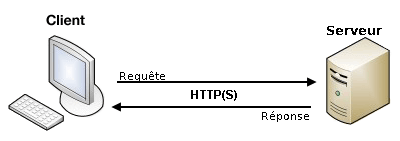
\includegraphics[width=0.6\textwidth,height=\textheight]{images/client-serveur.png}
\caption{Architecture client serveur}
\end{figure}

\end{center}

Les inventeurs du Web,
\href{https://interstices.info/les-debuts-du-web-sous-loeil-du-w3c/}{Tim
Berners-Lee} et
\href{https://fr.wikipedia.org/wiki/Robert_Cailliau}{Robert Caillau} ont
défini au
\href{https://fr.wikipedia.org/wiki/Organisation_europ\%C3\%A9enne_pour_la_recherche_nucl\%C3\%A9aire}{CERN}
entre 1989 et 1991 ses trois piliers
\href{https://developer.mozilla.org/fr/docs/Glossaire/HTTP}{HTTP},
\url{URL} et \url{HTML}.

\begin{cours}{}

\begin{itemize}
\tightlist
\item
  Dans un échange sur le Web, le \textbf{client} envoie une demande ou
  \textbf{requête} à l'aide d'un logiciel appelé \textbf{navigateur}
  \footnote{Note : Ne pas confondre navigateurs comme Firefox, Edge,
    Chrome et moteurs de recherche comme Qwant, Google search, Bing} :
  le \textbf{serveur} est un logiciel installé sur une machine reliée en
  réseau à la machine du client.
\item
  Le protocole
  \href{https://developer.mozilla.org/fr/docs/Glossaire/HTTP}{HTTP},
  acronyme d'\passthrough{\lstinline!Hypertext Transfer Protocol!}, est
  un protocole de la couche application qui décrit le format des
  échanges de données entre un client et un serveur sur le Web. Un
  échange HTTP s'établit selon le schéma suivant :

  \begin{itemize}
  \tightlist
  \item
    Le client saisit une
    \href{https://developer.mozilla.org/fr/docs/Glossaire/URL}{URL} dans
    la barre d'adresse du navigateur, elle est résolue en adresse
    \href{https://developer.mozilla.org/fr/docs/Glossaire/IP_Address}{IP}
    par le service
    \href{https://developer.mozilla.org/fr/docs/Glossaire/DNS}{DNS}.
  \item
    Mise en place d'une connexion TCP entre le client et le serveur.
  \item
    Le client envoie une requête HTTP (format texte lisible par un
    humain).
  \item
    Le serveur retourne une réponse HTTP, lue par le client. S'il y a un
    contenu, il est affiché par le navigateur du client.
  \item
    Fermeture ou réutilisation (paramètre
    \passthrough{\lstinline!Keep-alive!}) de la connexion pour les
    requêtes suivantes.
  \end{itemize}
\end{itemize}

Le protocole
\href{https://developer.mozilla.org/fr/docs/Glossaire/HTTP}{HTTP} n'est
pas sécurisé par défaut, il peut l'être par l'ajout du protocole SSL ou
TLS et on désigne par
\href{https://developer.mozilla.org/fr/docs/Glossaire/https}{HTTPS} sa
version sécurisée.
\href{https://developer.mozilla.org/fr/docs/Glossaire/HTTP}{HTTP} est un
standard normalisé par
l'\href{https://developer.mozilla.org/fr/docs/Glossaire/IETF}{IETF}
comme les protocoles d'internet
\href{https://developer.mozilla.org/fr/docs/Glossaire/TCP}{TCP} et
\href{https://developer.mozilla.org/fr/docs/Glossaire/IP_Address}{IP}.

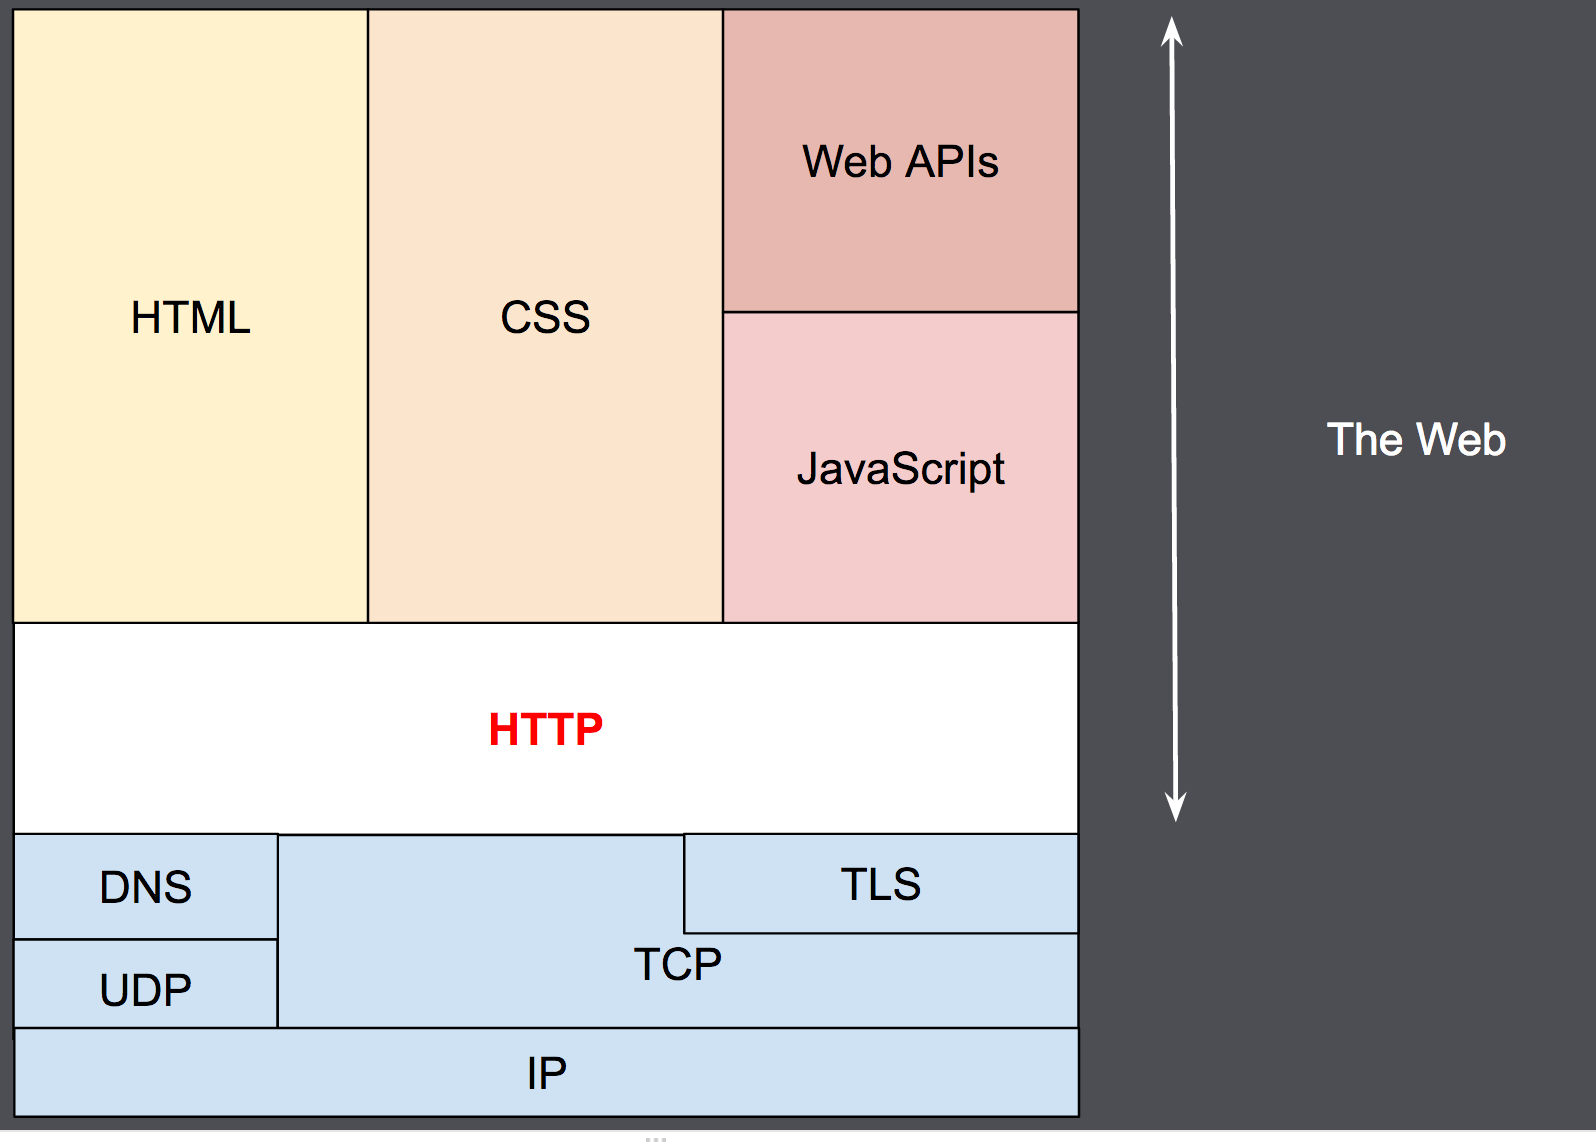
\includegraphics[width=0.5\textwidth,height=\textheight]{images/HTTP_layers.png}\\
\emph{Source :
\url{https://developer.mozilla.org/fr/docs/Web/HTTP/Aper\%C3\%A7u}}

\begin{itemize}
\tightlist
\item
  Une adresse
  \href{https://developer.mozilla.org/fr/docs/Glossaire/URL}{URL} pour
  \passthrough{\lstinline!Uniform Ressource Locator!} identifie une
  ressource sur le Web. La syntaxe des
  \href{https://developer.mozilla.org/fr/docs/Glossaire/URL}{URL} est
  standardisée, par exemple décomposons :\\
  \url{https://www.gnu.org/gnu/linux-and-gnu.fr.html} :

  \begin{itemize}
  \tightlist
  \item
    le protocole est \passthrough{\lstinline!https!} ;
  \item
    le nom de domaine sur Internet du serveur Web est
    \passthrough{\lstinline!gnu.org!}.\\
    \passthrough{\lstinline!www.gnu.org!} est un sous-domaine servant
    d'alias pour le dossier public du serveur ;
  \item
    \passthrough{\lstinline!gnu/linux-and-gnu.fr.html!} est le chemin
    vers la ressource sur le serveur : le fichier
    \passthrough{\lstinline!linux-and-gnu.fr.html!} qui se trouve dans
    le dossier public \passthrough{\lstinline!gnu!}.
  \end{itemize}
\item
  \href{https://developer.mozilla.org/fr/docs/Glossaire/HTML}{HTML} pour
  \passthrough{\lstinline!Hypertext Markup Language!} est le langage de
  description des documents textes disponibles sur le Web qui sont
  reliées entre eux par des des liens hypertextes. Il s'agit d'un
  langage à balises. En pratique, d'autres types de ressources sont
  accessible sur le Web par une
  \href{https://developer.mozilla.org/fr/docs/Glossaire/URL}{URL} : des
  images, des fichiers de données (aux formats CSV, JSON \ldots), des
  videos \ldots{} Par ailleurs les pages sont désormais réalisées en
  combinant
  \href{https://developer.mozilla.org/fr/docs/Glossaire/HTML}{HTML} avec
  \href{https://developer.mozilla.org/fr/docs/Glossaire/CSS}{CSS} pour
  la mise en forme, le positionnement, certains effets visuels et
  \href{https://developer.mozilla.org/fr/docs/Glossaire/JavaScript}{Javascript}
  pour la programmation évenementielle nécessaire à l'interactivité côté
  client.
\end{itemize}

\href{images/anatomie-element-html.png}{Un élément HTM \emph{source :}
https://developer.mozilla.org/fr/docs/Glossaire/HTML}\\

\end{cours}

\begin{exercice}{}

\emph{QCM} de type E3C2.

\begin{enumerate}
\def\labelenumi{\arabic{enumi}.}
\tightlist
\item
  Quelle est le code HTML permettant de créer un lien hypertexte dans un
  document écrit en
  \href{https://developer.mozilla.org/fr/docs/Glossaire/HTML}{HTML} ?

  \begin{itemize}
  \tightlist
  \item
    Réponse A : \passthrough{\lstinline!<a\\>http://tip-top.fr </a>!}
  \item
    Réponse B :
    \passthrough{\lstinline!<a href="http://tip-top.fr">Site du TIP-TOP</a>!}
  \item
    Réponse C : \passthrough{\lstinline!<a name="http://tip.top.fr</a>!}
  \end{itemize}
\item
  Comment s'appelle le service qui permet de faire le lien entre une IP
  et un nom de domaine ?

  \begin{itemize}
  \tightlist
  \item
    Réponse A : DNS
  \item
    Réponse B : ARP
  \item
    Réponse C : HTTP
  \item
    Réponse D : Internet
  \end{itemize}
\end{enumerate}

\end{exercice}

\begin{exercice}{}

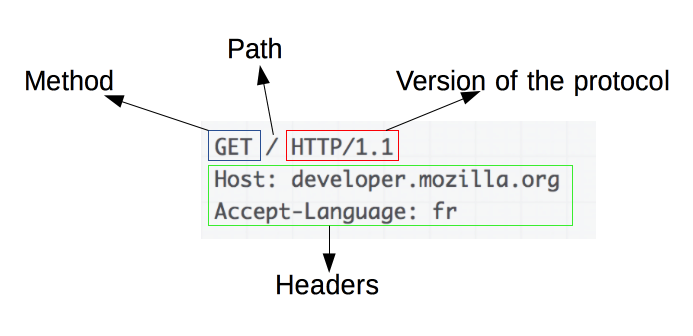
\includegraphics[width=0.5\textwidth,height=\textheight]{images/HTTP_Request.png}\\
\emph{Source :
\url{https://developer.mozilla.org/fr/docs/Web/HTTP/Aper\%C3\%A7u}}

\begin{enumerate}
\def\labelenumi{\arabic{enumi}.}
\item
  Avec un navigateur Web, demander la page d'adresse\\
  \url{http://frederic-junier.org/NSI/sandbox/index.html}.\\
  Ouvrir la barre d'outils de développement en appuyant sur la touche de
  fonction \passthrough{\lstinline!F12!} et sélectionner l'onglet
  Réseau. On peut voir les entêtes de la requête et de la réponse HTTP.

  \begin{itemize}
  \tightlist
  \item
    Que représente le code d'état de la réponse HTTP ?
  \item
    Quelles informations sur le client sont transmises au serveur dans
    l'entête de la requête ?
  \item
    Quelles informations sur le serveur sont transmises au client dans
    l'entête de la réponse ?
  \item
    Effectuer une nouvelle requête avec
    l'\href{https://developer.mozilla.org/fr/docs/Glossaire/URL}{URL}
    \url{http://frederic-junier.org/NSI/sandbox/}. Quelle différence
    avec la requête initiale ?
  \item
    Effectuer une nouvelle requête avec
    l'\href{https://developer.mozilla.org/fr/docs/Glossaire/URL}{URL}
    \url{https://frederic-junier.org/NSI/sandbox/}. Quelle différence
    avec la requête initiale peut-on observer dans la barre d'adresse du
    navigateur ?
  \item
    Effectuer une nouvelle requête avec
    l'\href{https://developer.mozilla.org/fr/docs/Glossaire/URL}{URL}
    \url{http://frederic-junier.org/NSI/Sandbox/index.html}. Quel est le
    code d'état de la réponse ? Explication ?
  \item
    Effectuer une nouvelle requête avec
    l'\href{https://developer.mozilla.org/fr/docs/Glossaire/URL}{URL}
    \url{http://frederic-junier.org/NSI/interdit}. Quel est le code
    d'état de la réponse ? Explication ?
  \end{itemize}
\item
  Le site \url{https://httpie.org/} propose un client HTTP en ligne de
  commandes permettant de décomposer les requêtes HTTP en précisant la
  méthode et l'URL de la ressource demandée.

  \begin{itemize}
  \tightlist
  \item
    Ouvrir la page \url{https://httpie.org/run}
  \item
    Saisir la commande
    \passthrough{\lstinline!http -v GET https://frederic-junier.org/NSI/sandbox/index.html!}.
    Décrire le fonctionnement de la méthode
    \passthrough{\lstinline!GET!} du protocole
    \passthrough{\lstinline!HTTP!} : formats de la requête et de la
    réponse.
  \item
    Saisir la commande
    \passthrough{\lstinline!http -v HEAD https://frederic-junier.org/NSI/sandbox/index.html!}.
    Décrire le fonctionnement de la méthode
    \passthrough{\lstinline!HEAD!} du protocole
    \passthrough{\lstinline!HTTP!} : formats de la requête et de la
    réponse.
  \item
    Saisir la commande
    \passthrough{\lstinline!http -v PUT https://frederic-junier.org/NSI/sandbox/index.html hello=wolrd!}.
    Quel résultat obtient-on ? Explication \footnote{Note : Méthodes
      HTTP : voir
      \url{https://developer.mozilla.org/fr/docs/Web/HTTP/M\%C3\%A9thode}}
    ?
  \end{itemize}
\end{enumerate}

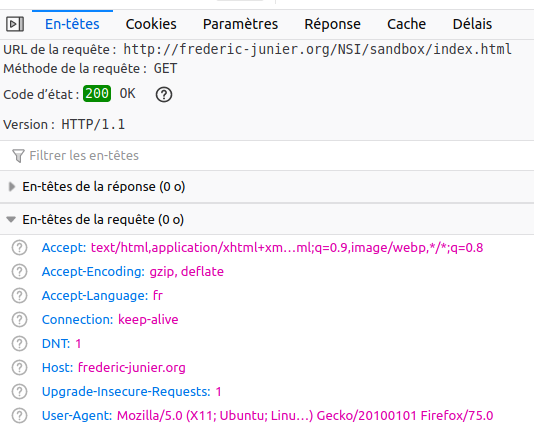
\includegraphics[width=0.5\textwidth,height=\textheight]{images/header-http1.png}\\

\end{exercice}

\hypertarget{passage-de-paramuxe8tres-dans-une-url}{%
\subsection{Passage de paramètres dans une
URL}\label{passage-de-paramuxe8tres-dans-une-url}}

\begin{exercice}{}

Ouvrir un navigateur Web.

\begin{enumerate}
\def\labelenumi{\arabic{enumi}.}
\item
  Demander la page d'adresse
  \href{https://frederic-junier.org/NSI/sandbox/accueil.php}{http://frederic-junier.org/NSI/sandbox/accueil.php}

  Quel est l'affichage obtenu ?
\item
  Demander la page d'adresse\\
  \href{https://frederic-junier.org/NSI/sandbox/accueil.php}{http://frederic-junier.org/NSI/sandbox/accueil.php?nom=Turing\&prenom=Alan}

  Quel est l'affichage obtenu ? Ouvrir les outils de développement avec
  \passthrough{\lstinline!F12!} puis sélectionner les onglets
  \passthrough{\lstinline!Réseau!} et
  \passthrough{\lstinline!Paramètres!}.

  \textbf{La partie \passthrough{\lstinline!?nom=Turing\&prenom=Alan!}
  de l'\href{https://developer.mozilla.org/fr/docs/Glossaire/URL}{URL}
  est une \emph{chaîne de requête}, elle commence par le symbole
  \passthrough{\lstinline!?!} puis contient une liste de paires
  \passthrough{\lstinline!nom=valeur!} séparées par un symbole
  esperluette \passthrough{\lstinline!\&!}. Ces paramètres ne font pas
  partie de l'adresse de la ressource mais sont une façon pour le client
  de transmettre des informations au serveur.}

  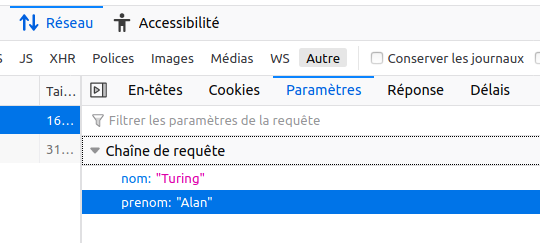
\includegraphics[width=0.5\textwidth,height=\textheight]{images/parametres1.png}\\
\item
  Remplacer Turing par votre nom et Alan par votre prénom dans
  l'\href{https://developer.mozilla.org/fr/docs/Glossaire/URL}{URL}
  précédente. Que peut-on remarquer ? À votre avis, que se passe-t-il
  sur le serveur lorsqu'il reçoit la requête HTTP ?
\item
  Voici le contenu du fichier \passthrough{\lstinline!accueil.php!} sur
  le serveur. S'agit-il d'un texte écrit en
  \href{https://developer.mozilla.org/fr/docs/Glossaire/HTML}{HTML} ?
  Faire une recherche sur la signification de l'acronyme
  \href{https://developer.mozilla.org/fr/docs/Glossaire/PHP}{PHP}.
\end{enumerate}

\begin{lstlisting}[language=PHP]
 <!DOCTYPE html>
<html lang="fr">
<head>
  <title>Accueil </title>
  <meta charset="utf-8">    
</head> 
<body>
<h1>
<?php  
echo "Bienvenue " . $_GET['prenom'] . " " .  $_GET['nom'] ;
?>
</h1>
</body>
</html> 
\end{lstlisting}

\begin{enumerate}
\def\labelenumi{\arabic{enumi}.}
\setcounter{enumi}{3}
\tightlist
\item
  Enregistrer
  l'\href{https://developer.mozilla.org/fr/docs/Glossaire/URL}{URL}
  testée précédemment dans les marque-pages du navigateur. Ouvrir un
  autre onglet et cliquer sur le signet enregistré. Retrouve-t-on la
  même page Web ?
\end{enumerate}

\end{exercice}

\hypertarget{formulaire-et-passage-de-paramuxe8tres}{%
\section{Formulaire et passage de
paramètres}\label{formulaire-et-passage-de-paramuxe8tres}}

\hypertarget{un-premier-exemple}{%
\subsection{Un premier exemple}\label{un-premier-exemple}}

\begin{exemple}{}

\begin{enumerate}
\def\labelenumi{\arabic{enumi}.}
\item
  Ouvrir avec un navigateur Web la page
  d'\href{https://developer.mozilla.org/fr/docs/Glossaire/URL}{URL} :

  \url{http://frederic-junier.org/NSI/sandbox/formulaire-get.html}

  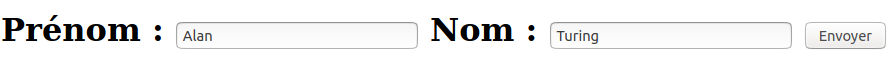
\includegraphics{images/formulaire1.png}\\

  \begin{itemize}
  \tightlist
  \item
    Cliquer sur le bouton \passthrough{\lstinline!Envoyer!}. Que se
    passe-t-il ? Rafraîchir la page avec \passthrough{\lstinline!F5!}.
    Que se passe-t-il ?
  \item
    Changer les valeurs des champs \passthrough{\lstinline!Prénom!} et
    \passthrough{\lstinline!Nom!} du formulaire puis cliquer sur le
    bouton \passthrough{\lstinline!Envoyer!}. Que se passe-t-il ?
  \item
    Ouvrir la fenêtre des outils de développement et afficher dans
    l'onglet Réseau l'entête de la requête HTTP qui devrait ressembler à
    celui-ci :
  \end{itemize}

  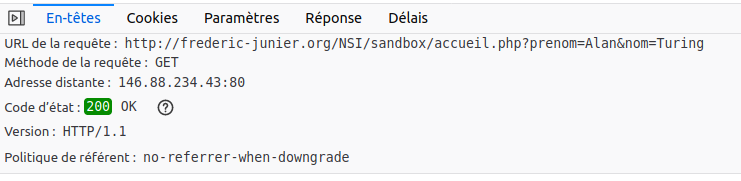
\includegraphics[width=0.8\textwidth,height=\textheight]{images/entete-get.png}\\

  Sélectionner l'onglet Paramètres et vérifier qu'on obtient les
  paramètres tranmise dans
  l'\href{https://developer.mozilla.org/fr/docs/Glossaire/URL}{URL}{[}URL\}
  dans la chaîne de requête comme dans l'exercice 3.

  \begin{itemize}
  \tightlist
  \item
    Afficher le code source de la page
    \passthrough{\lstinline!formulaire-get.html!} avec le raccourci
    clavier \passthrough{\lstinline!CRTL + U!}. On devrait obtenir le
    texte ci-dessous :
  \end{itemize}

\begin{lstlisting}[language=HTML]
<!DOCTYPE html>

<html lang="fr">

<head>
<title>Formulaire HTML </title>
<meta charset="utf-8">    
</head> 
<body>

   <form action = "accueil.php" method="GET">        
      <label for="id_prenom">Prénom :</label>
      <input type="text" id="id_prenom" name="prenom" value="Alan">
      <label for="id_nom">Nom :</label>
      <input type="text" id="id_nom" name="nom" value="Turing">
      <button type="submit" id="bouton">Envoyer</button>
   </form>

</body>
</html> 
\end{lstlisting}
\item
  Ouvrir avec un navigateur Web la page
  d'\href{https://developer.mozilla.org/fr/docs/Glossaire/URL}{URL} :

  \url{http://frederic-junier.org/NSI/sandbox/formulaire-post.html}

  \begin{itemize}
  \tightlist
  \item
    Cliquer sur le bouton \passthrough{\lstinline!Envoyer!}. Que se
    passe-t-il ?
  \item
    Changer les valeurs des champs \passthrough{\lstinline!Prénom!} et
    \passthrough{\lstinline!Nom!} du formulaire puis cliquer sur le
    bouton \passthrough{\lstinline!Envoyer!}. Que se passe-t-il ?
    Observe-t-on un changement dans
    l'\href{https://developer.mozilla.org/fr/docs/Glossaire/URL}{URL} de
    la requête ? dans son entête ?
  \item
    Rafraîchir la nouvelle avec \passthrough{\lstinline!F5!}. Que se
    passe-t-il ?
  \end{itemize}

  
\includegraphics[width=0.7\textwidth,height=\textheight]{images/avertissement-post.png}\\

  \begin{itemize}
  \tightlist
  \item
    Ouvrir la fenêtre des outils de développement et afficher dans
    l'onglet Réseau l'entête de la requête HTTP qui devrait ressembler à
    celui-ci :
  \end{itemize}

  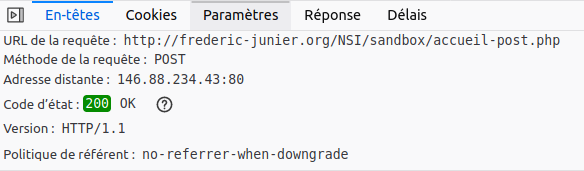
\includegraphics[width=0.6\textwidth,height=\textheight]{images/entete-post.png}\\

  Sélectionner l'onglet Paramètres et vérifier qu'on retrouve les
  paramètres transmis dans
  l'\href{https://developer.mozilla.org/fr/docs/Glossaire/URL}{URL}.
  Quelle différence par rapport à la méthode vue en question 1 ?

  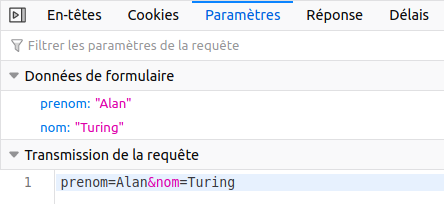
\includegraphics[width=0.4\textwidth,height=\textheight]{images/parametres2.png}\\

  \begin{itemize}
  \tightlist
  \item
    Afficher le code source de la page
    \passthrough{\lstinline!formulaire-get.html!} avec le raccourci
    clavier \passthrough{\lstinline!CRTL + U!}. Quels sont les deux
    changements par rapport au code de
    \passthrough{\lstinline!formulaire-post.html!} ?
  \end{itemize}
\end{enumerate}

\end{exemple}

\hypertarget{muxe9thodes-de-passage-des-paramuxe8tres-get-ou-post}{%
\subsection{Méthodes de passage des paramètres : GET ou
POST}\label{muxe9thodes-de-passage-des-paramuxe8tres-get-ou-post}}

\begin{cours}{}

En \href{https://developer.mozilla.org/fr/docs/Glossaire/HTML}{HTML}, un
formulaire est un élément qui permet de transmettre des informations à
un serveur Web. Il est composé d'un élément
\passthrough{\lstinline!<form action="http://domaine/cible" method="GET" >!}
qui contient un ou plusieurs widgets, des éléments
\href{https://developer.mozilla.org/fr/docs/Glossaire/HTML}{HTML}
permettant de saisir les entrées du client et au moins un élément
\passthrough{\lstinline!<button type="submit>Bouton d'envoi</button>!}.
Un clic sur ce dernier déclenche l'exécution d'une requête
\href{https://developer.mozilla.org/fr/docs/Glossaire/HTTP}{HTTP} qui va
transmettre les données saisies seln les valeurs des attibuts
\passthrough{\lstinline!action!} et \passthrough{\lstinline!method!} de
l'élément \passthrough{\lstinline!<form>!} :

\begin{itemize}
\tightlist
\item
  \passthrough{\lstinline!action!} a pour valeur
  l'\href{https://developer.mozilla.org/fr/docs/Glossaire/URL}{URL} du
  fichier auquel sera envoyé le formulaire. Ce fichier est un programme
  écrit dans un langage de script comme
  \href{https://developer.mozilla.org/fr/docs/Glossaire/PHP}{PHP} ou
  \href{https://docs.python.org/3.7/library/cgi.html}{Python}, qui va
  prendre en entrée les paramètres du formulaire transmis par le client,
  les traiter et générer la page Web en
  \href{https://developer.mozilla.org/fr/docs/Glossaire/HTML}{HTML} qui
  lui sera retournée.
\item
  \passthrough{\lstinline!method!} peut prendre deux valeurs
  \href{https://developer.mozilla.org/fr/docs/Web/HTTP/M\%C3\%A9thode/GET}{GET}
  ou
  \href{https://developer.mozilla.org/fr/docs/Web/HTTP/M\%C3\%A9thode/POST}{POST}
  (en minuscule ou majuscule), ce sont les deux modes de transmission
  des paramètres du formulaire qui sont deux méthodes distinctes du
  protocole
  \href{https://developer.mozilla.org/fr/docs/Glossaire/HTTP}{HTTP} :

  \begin{itemize}
  \tightlist
  \item
    avec la méthode
    \href{https://developer.mozilla.org/fr/docs/Web/HTTP/M\%C3\%A9thode/GET}{GET}
    , les données du formulaire sont assemblées dans une chaîne de
    paires \passthrough{\lstinline!nom=valeur!} séparées par le symbole
    \passthrough{\lstinline!\&!} qui est ajoutée à la fin de
    l'\href{https://developer.mozilla.org/fr/docs/Glossaire/URL}{URL}
    après un symbole \passthrough{\lstinline!?!}.
  \item
    avec la méthode
    \href{https://developer.mozilla.org/fr/docs/Web/HTTP/M\%C3\%A9thode/POST}{POST}
    les données du formulaire sont transmises toujours dans le corps de
    la requête. Les données n'apparaissent donc pas dans
    l'\href{https://developer.mozilla.org/fr/docs/Glossaire/URL}{URL} de
    la requête.
  \end{itemize}
\end{itemize}

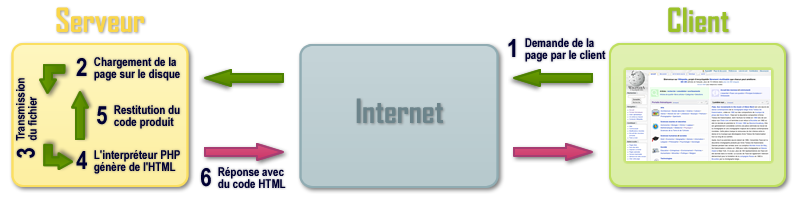
\includegraphics[width=0.8\textwidth,height=\textheight]{images/Php_arch_shema.png}\\

Le formulaire du fichier \passthrough{\lstinline!formulaire-get.html!}
de l'exemple 1 contient deux widgets \passthrough{\lstinline!<input>!}.
Chacun va fournir un couple \passthrough{\lstinline!nom=valeur!}, le nom
est désigné par l'attibut \passthrough{\lstinline!name!} et la valeur
par le texte saisi dans l'élément \passthrough{\lstinline!<input>!}.
Chacun est associépar son attribut \passthrough{\lstinline!id!} à une
étiquette contenue dans un élément \passthrough{\lstinline!<label>!}.

Caractéristiques de la méthode
\href{https://developer.mozilla.org/fr/docs/Web/HTTP/M\%C3\%A9thode/GET}{GET}
:

\begin{itemize}
\tightlist
\item
  Toutes les informations transmises, le sont en clair dans
  l'\href{https://developer.mozilla.org/fr/docs/Glossaire/URL}{URL}.
  Celle-ci est limitée en taille donc la méthode
  \href{https://developer.mozilla.org/fr/docs/Web/HTTP/M\%C3\%A9thode/GET}{GET}
  ne peut pas être utilisée pour transmettre des informations trop
  longues.
\item
  La méthode
  \href{https://developer.mozilla.org/fr/docs/Web/HTTP/M\%C3\%A9thode/GET}{GET}
  est constituée juste d'un entête, elle n'a pas de corps.
\item
  Elle ne modifie pas l'état du serveur, elle est utilisée uniquement
  pour demander une ressource. Un exemple classique d'utilisation est la
  formulation d'une requête à l'aide du formulaire d'un moteur de
  recherche.
  L'\href{https://developer.mozilla.org/fr/docs/Glossaire/URL}{URL}
  générée peut être utilisée plusieurs fois et conservée comme
  marque-page.
\end{itemize}

Caractéristiques de la méthode
\href{https://developer.mozilla.org/fr/docs/Web/HTTP/M\%C3\%A9thode/POST}{POST}
:

\begin{itemize}
\tightlist
\item
  Les données envoyées peuvent modifier l'état du serveur. Les requêtes
  \href{https://developer.mozilla.org/fr/docs/Web/HTTP/M\%C3\%A9thode/POST}{POST}
  sont utilisées pour les modifications de bases de données sur le
  serveur (achats, réservation, transfert de fichiers \ldots)
\item
  TLes données sont transmises dans le corps de la requête, il n'y a pas
  de restriction de taille. Elles peuvent être de tout type :
  url-encodées (chaîne de paires \passthrough{\lstinline!nom=valeur!}),
  ou binaires. C'est précisé dans le champ
  \passthrough{\lstinline!Content-type!} de l'entête comme pour une
  répone
  \href{https://developer.mozilla.org/fr/docs/Glossaire/HTTP}{HTTP}.
\item
  Les donnnées n'apparaissent pas dans
  l'\href{https://developer.mozilla.org/fr/docs/Glossaire/URL}{URL},
  néanmoins, si le protocole
  \href{https://developer.mozilla.org/fr/docs/Glossaire/HTTP}{HTTP} est
  employé sans chiffrement, il suffit d'intercepter la requête pour
  accéder aux données en clair.
\item
  Chaque utilisation de
  l'\href{https://developer.mozilla.org/fr/docs/Glossaire/URL}{URL}
  d'envoi modifie l'état du serveur, c'est pourquoi une fenêtre
  d'avertissement apparaît lorsqu'on veut renvoyer les données d'un
  formulaire avec
  \href{https://developer.mozilla.org/fr/docs/Web/HTTP/M\%C3\%A9thode/POST}{POST}.
\end{itemize}

\end{cours}

\begin{exercice}{}

\emph{QCM} de type E3C2.

\begin{enumerate}
\def\labelenumi{\arabic{enumi}.}
\item
  Parmi les réponses suivantes, que permet d'effectuer la méthode
  \href{https://developer.mozilla.org/fr/docs/Web/HTTP/M\%C3\%A9thode/POST}{POST}
  du protocole
  \href{https://developer.mozilla.org/fr/docs/Glossaire/HTTP}{HTTP}~?

  \begin{itemize}
  \tightlist
  \item
    Réponse A : Définir le style d'une page web
  \item
    Réponse B : Pirater des données bancaire
  \item
    Réponse C : Envoyer une page web vers le client
  \item
    Réponse D : Envoyer les données saisies dans un formulaire HTML vers
    un serveur
  \end{itemize}
\item
  Un site internet utilise une requête
  \href{https://developer.mozilla.org/fr/docs/Glossaire/HTTP}{HTTP} avec
  la méthode
  \href{https://developer.mozilla.org/fr/docs/Web/HTTP/M\%C3\%A9thode/POST}{POST}
  pour transmettre les données d'un formulaire. Laquelle des
  affirmations suivantes est \textbf{incorrecte}~?

  \begin{itemize}
  \tightlist
  \item
    Réponse A : les données envoyées ne sont pas visibles
  \item
    Réponse B : il est possible de transmettre des données de type
    binaire
  \item
    Réponse C : les données transmises sont cryptées
  \item
    Réponse D : il n'y a pas de restriction de longueur pour les données
    transmises
  \end{itemize}
\item
  Un internaute clique sur un lien qui envoie la requête
  \href{https://developer.mozilla.org/fr/docs/Glossaire/HTTP}{HTTP}
  suivante à un serveur~:

  \passthrough{\lstinline!http://jaimelaneige.com/ma\_planche/traitement.php?nom=Snow\&prenom=Jon!}

  Que demande cette requête au serveur ?

  \begin{itemize}
  \tightlist
  \item
    Réponse A : de renvoyer le fichier traitement.php en identifiant nom
    et prénom à Snow et Jon
  \item
    Réponse B : d'exécuter le fichier traitement.php en identifiant nom
    et prénom à Snow et Jon
  \item
    Réponse C : d'indiquer si Jon Snow a bien pris son traitement
  \item
    Réponse D : de renvoyer le fichier traitement.php en affichant
    prénom et nom : Jon
  \end{itemize}
\end{enumerate}

\end{exercice}

\hypertarget{eluxe9ments-de-formulaire}{%
\subsection{Eléments de formulaire}\label{eluxe9ments-de-formulaire}}

\begin{cours}{}

\begin{enumerate}
\def\labelenumi{\arabic{enumi}.}
\item
  Le principal élément permettant la saisie de données dans un champ de
  formulaire
  \href{https://developer.mozilla.org/fr/docs/Glossaire/HTML}{HTML} est
  \passthrough{\lstinline!<input>!}. Son attribut
  \passthrough{\lstinline!type!} permet de vérifier que les données
  saisies correspondent au type attendu.

  \begin{longtable}[]{@{}ll@{}}
  \toprule
  \begin{minipage}[b]{0.47\columnwidth}\raggedright
  Type\strut
  \end{minipage} & \begin{minipage}[b]{0.47\columnwidth}\raggedright
  Exemple de syntaxe\strut
  \end{minipage}\tabularnewline
  \midrule
  \endhead
  \begin{minipage}[t]{0.47\columnwidth}\raggedright
  Texte\strut
  \end{minipage} & \begin{minipage}[t]{0.47\columnwidth}\raggedright
  \passthrough{\lstinline!<input type="text"  name="t"  value="Défaut">!}\strut
  \end{minipage}\tabularnewline
  \begin{minipage}[t]{0.47\columnwidth}\raggedright
  Email\strut
  \end{minipage} & \begin{minipage}[t]{0.47\columnwidth}\raggedright
  \passthrough{\lstinline!<input type="email"  name="a"  value="defaut@defaut.fr">!}\strut
  \end{minipage}\tabularnewline
  \begin{minipage}[t]{0.47\columnwidth}\raggedright
  Nombre\strut
  \end{minipage} & \begin{minipage}[t]{0.47\columnwidth}\raggedright
  \passthrough{\lstinline!<input type="number"  name="n"  value="1" min="0" max="10">!}\strut
  \end{minipage}\tabularnewline
  \begin{minipage}[t]{0.47\columnwidth}\raggedright
  Mot de passe\strut
  \end{minipage} & \begin{minipage}[t]{0.47\columnwidth}\raggedright
  \passthrough{\lstinline!<input type="password"   name="pwd">!}\strut
  \end{minipage}\tabularnewline
  \begin{minipage}[t]{0.47\columnwidth}\raggedright
  Cases à cocher\strut
  \end{minipage} & \begin{minipage}[t]{0.47\columnwidth}\raggedright
  \passthrough{\lstinline!<input type="checkbox"  name="carrots"  value="carrots">!}\strut
  \end{minipage}\tabularnewline
  \begin{minipage}[t]{0.47\columnwidth}\raggedright
  Bouton radio (choix exclusif)\strut
  \end{minipage} & \begin{minipage}[t]{0.47\columnwidth}\raggedright
  \passthrough{\lstinline!<input type="radio"  value="soup"  name="meal">!}\strut
  \end{minipage}\tabularnewline
  \bottomrule
  \end{longtable}
\item
  L'élément \passthrough{\lstinline!<textarea>!} permet de saisir un
  texte de longueur arbitraire et \passthrough{\lstinline!<select>!}
  permet de définir une liste déroulante.
\item
  Le bouton de soumission d'un formulaire est représenté par un élément
  de la forme
  \passthrough{\lstinline!<button type="submit">Envoyer</button>!}.
\end{enumerate}

La page
\url{https://developer.mozilla.org/fr/docs/Web/Guide/HTML/Formulaires/Les_blocs_de_formulaires_natifs}
décrit les principaux widgets de formulaire et la page
\url{https://www.w3schools.com/html/html_form_elements.asp} permet de
les tester.

\end{cours}

\begin{exercice}{}

\begin{enumerate}
\def\labelenumi{\arabic{enumi}.}
\item
  Ouvrir dans un navigateur Web la page dont
  l'\href{https://developer.mozilla.org/fr/docs/Glossaire/URL}{URL} est
  :\\
  \url{https://repl.it/@fredericjunier/NSI-formulaire-exo5-radio}.

  \begin{itemize}
  \tightlist
  \item
    Cliquer sur \passthrough{\lstinline!Restart!} pour lancer le
    serveur, remplir le formulaire contenu dans le fichier
    \passthrough{\lstinline!index.php!} et envoyer les données. Quelle
    méthode est utilisée pour le passage des paramètres du formulaire ?
  \item
    Modifier les codes sources des fichiers
    \passthrough{\lstinline!index.php!} et
    \passthrough{\lstinline!navigateur.php!} pour changer la méthode de
    passage des paramètres du formulaire. En
    \href{https://developer.mozilla.org/fr/docs/Glossaire/PHP}{PHP}, on
    récupère la valeur du paramètre \passthrough{\lstinline!nom!} avec
    \passthrough{\lstinline!$\_GET['nom']!} si la méthode est
    \href{https://developer.mozilla.org/fr/docs/Web/HTTP/M\%C3\%A9thode/GET}{GET}
    ou \passthrough{\lstinline!$\_POST['nom']!} si c'est
    \href{https://developer.mozilla.org/fr/docs/Web/HTTP/M\%C3\%A9thode/POST}{POST}.
  \item
    Consulter la documentation sur l'élément de formulaire
    \passthrough{\lstinline!<select>!} contenue dans la page
    \url{https://www.w3schools.com/html/html_form_elements.asp} et
    remplacer les \passthrough{\lstinline!<input>!} de type
    \passthrough{\lstinline!radio!} du formulaire dans
    \passthrough{\lstinline!index.php!} par un élément
    \passthrough{\lstinline!<select>!} avec choix unique.
  \end{itemize}
\item
  Ouvrir dans un navigateur Web la page dont
  l'\href{https://developer.mozilla.org/fr/docs/Glossaire/URL}{URL} est
  :\\
  \url{https://repl.it/@fredericjunier/NSI-formulaire-exo5-checkbox}.

  \begin{itemize}
  \tightlist
  \item
    Cliquer sur \passthrough{\lstinline!Restart!} pour lancer le
    serveur, remplir le formulaire contenu dans le fichier
    \passthrough{\lstinline!index.php!} et envoyer les données. Quelle
    méthode est utilisée pour le passage des paramètres du formulaire ?
  \item
    Modifier les codes sources des fichiers
    \passthrough{\lstinline!index.php!} et
    \passthrough{\lstinline!langages.php!} pour changer la méthode de
    passage des paramètres du formulaire.
  \item
    Consulter la documentation sur l'élément de formulaire
    \passthrough{\lstinline!<select>!} contenue dans la page
    \url{https://www.w3schools.com/html/html_form_elements.asp} et
    remplacer les \passthrough{\lstinline!<input>!} de type
    \passthrough{\lstinline!checkbox!} du formulaire dans
    \passthrough{\lstinline!index.php!} par un élément
    \passthrough{\lstinline!<select>!} avec choix multiple.
  \end{itemize}
\item
  Ouvrir dans un navigateur Web la page dont
  l'\href{https://developer.mozilla.org/fr/docs/Glossaire/URL}{URL} est
  :\\
  \url{http://frederic-junier.org/NSI/sandbox/NSI-formulaire-exo5-login-get.html}.

  \begin{itemize}
  \tightlist
  \item
    La page présente un formulaire basique de connexion avec deux champs
    \passthrough{\lstinline!login!} et
    \passthrough{\lstinline!password!}. La valeur de l'identifiant est
    libre et le mot de passe est \passthrough{\lstinline!secret!}.
    Remplir le formulaire et envoyer les données. Quelle méthode de
    passage des paramètres est utilisée ? La transmission du mot de
    passe est-elle satisfaisante.
  \item
    Revenir sur la page du formulaire, ouvrir la fenêtre des outils de
    développement avec \passthrough{\lstinline!F12!} et modifier le code
    source pour que l'envoi du mot de passe soit sécurisé.
  \end{itemize}

  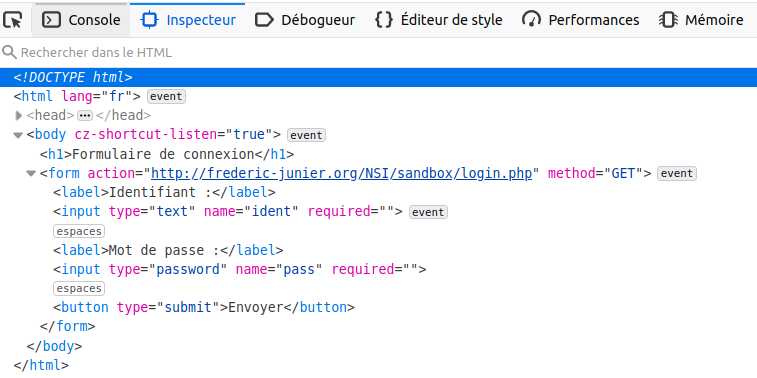
\includegraphics[width=0.6\textwidth,height=\textheight]{images/login.png}\\

  \begin{itemize}
  \tightlist
  \item
    Dans le schéma ci-dessous d'un échange Web sécurisé avec le
    protocole
    \href{https://developer.mozilla.org/fr/docs/Glossaire/https}{HTTPS},
    apparaît la notion de
    \href{https://developer.mozilla.org/fr/docs/Glossaire/Certificat_num\%C3\%A9rique}{certificat}.
    Quel est le rôle d'un
    \href{https://developer.mozilla.org/fr/docs/Glossaire/Certificat_num\%C3\%A9rique}{certificat}
    et comment est-il géré par le navigateur ?
  \end{itemize}

  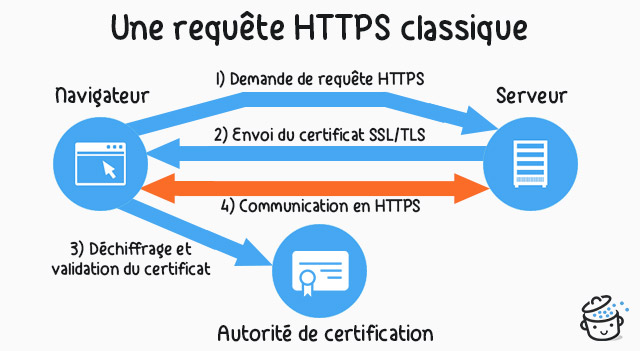
\includegraphics[width=0.6\textwidth,height=\textheight]{images/schema-requete-https.jpg}\\

  \emph{Source : \url{https://wpmarmite.com/wordpress-https/}}
\end{enumerate}

\end{exercice}

\end{document}
